\section{Characterization of the FBG-based FOS}
As described in the section~\ref{fbg}, it's possible to measure the relative humidity instead of the strain, if the coating of the fiber wire is moisture content. The secondary strain effect related to the so-called swelling effect of the polymer coating allows measuring the \gls{RH}~\cite{YEO_PI}. The key to effective humidity measurement is the choice of the thickness of the coating. In principle, any moisture-sensitive material or polymer could be used to build sensors. Still, the polyimide has a linear response to the humidity, and also it is commonly used for many industrial sensing applications (mainly capacitive sensors). The studies by Berruti~\cite{Berruti} and Yeo~\cite{YEO_PI} were used to determine which coating thickness should be used to get the best results. The main efforts were concentrated to optimize the design of the polyimide-coated FBG sensors in order to be able to measure in low temperatures. For example, Yeo et al. \cite{YEO_PI} studied different polyimide thicknesses to find out how the \gls{RH} sensitivity and response time varies with increasing thickness (see figure~\ref{fig:yeo}). The \gls{RH} sensitivity increases linearly with the coating thickness, so in principle, a better sensitivity would result in a better sensor.
\begin{figure}[!h]
\centering
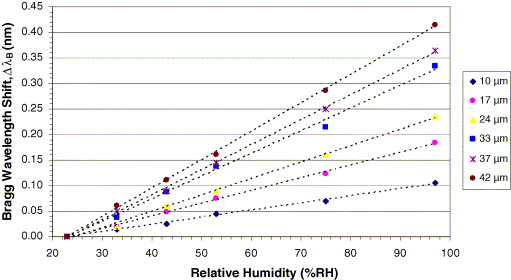
\includegraphics[width=0.75\columnwidth]{Chapter5/images/yeo_coating.jpg}
\caption{RH response of the sensors with different coating thicknesses from 23 to 97\%RH at constant room temperature~\cite{YEO_PI}}
\label{fig:yeo}
\end{figure}
The higher thickness reflects itself also in the increased time response as seen in the figure~\ref{fig:yeo2}. As for the \gls{STS} sensing system, the most crucial scenarios include an uncontrolled change of humidity which should be detected within minutes to conduct necessary actions in the control system. Therefore, the chosen coating thickness is between \SI{15}{\micro\metre} and \SI{20}{\micro\metre}, slightly higher than the first reported distributed sensing system implemented for the \gls{CMS} at \gls{CERN}, where \SI{10}{\micro\metre} were used. 
\begin{figure}[!h]
\centering
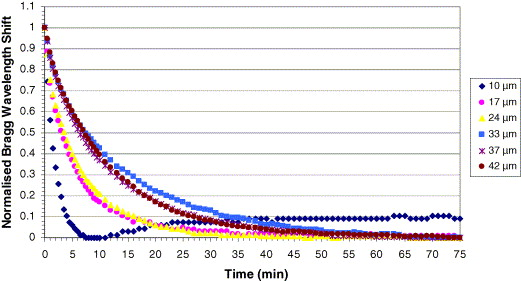
\includegraphics[width=0.75\columnwidth]{Chapter5/images/time_response_yeo.jpg}
\caption{Recovery time of the sensors from 75 to 33\%RH~\cite{YEO_PI}}
\label{fig:yeo2}
\end{figure}

In order to do so, two different designs were compared:
\begin{itemize}
    \item multiplexed version with 5 \glspl{FBG} inscribed in a germanium-doped fiber. The polyimide layer was applied in four steps, \SI{5}{\micro\metre} with \SI{1.25}{\micro\metre} uncertainty for each layer. In total the coating thickness was about \SI{20}{\micro\metre}$\pm$\SI{5}{\micro\metre}. The temperature compensation was ensured by a second \gls{FBG} array which measures only temperature (the sensitive part is in epoxy),
    \item the second design is a hygrometer with temperature and humidity sensors inscribed into one fiber. The coating thickness was chosen to be \SI{15}{\micro\metre}. The tested sensors are depicted in the figure~\ref{fig_single_photo}.
\end{itemize}

\begin{figure}[!h]
\centering
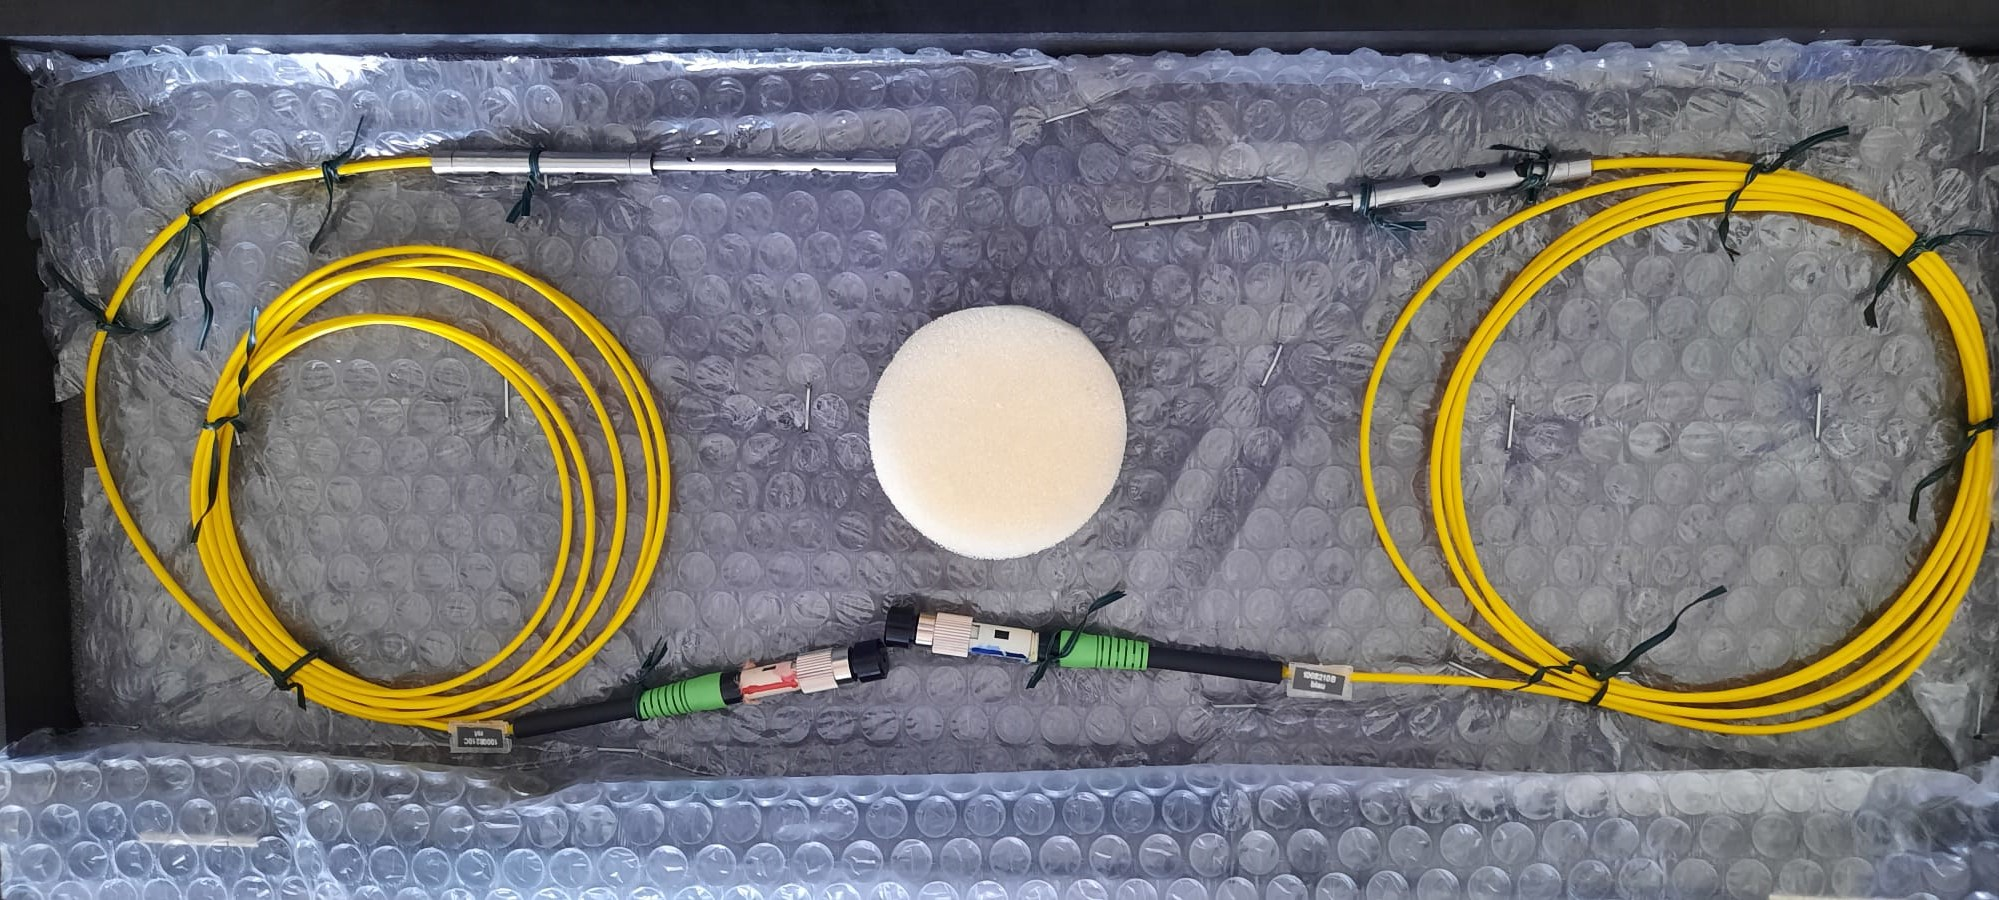
\includegraphics[width=0.75\columnwidth]{Chapter5/images/single1.jpeg}
\caption{Hygrometer (temperature and humidity sensitive \glspl{FBG} inscribed into the same fiber). The only difference between the two hygrometers in the photo is the diameter of the holder/packaging of the \gls{RH} sensitive \gls{FBG} (manufactured by AOS Electronics).}
\label{fig_single_photo}
\end{figure}

\begin{figure}[!h]
\centering
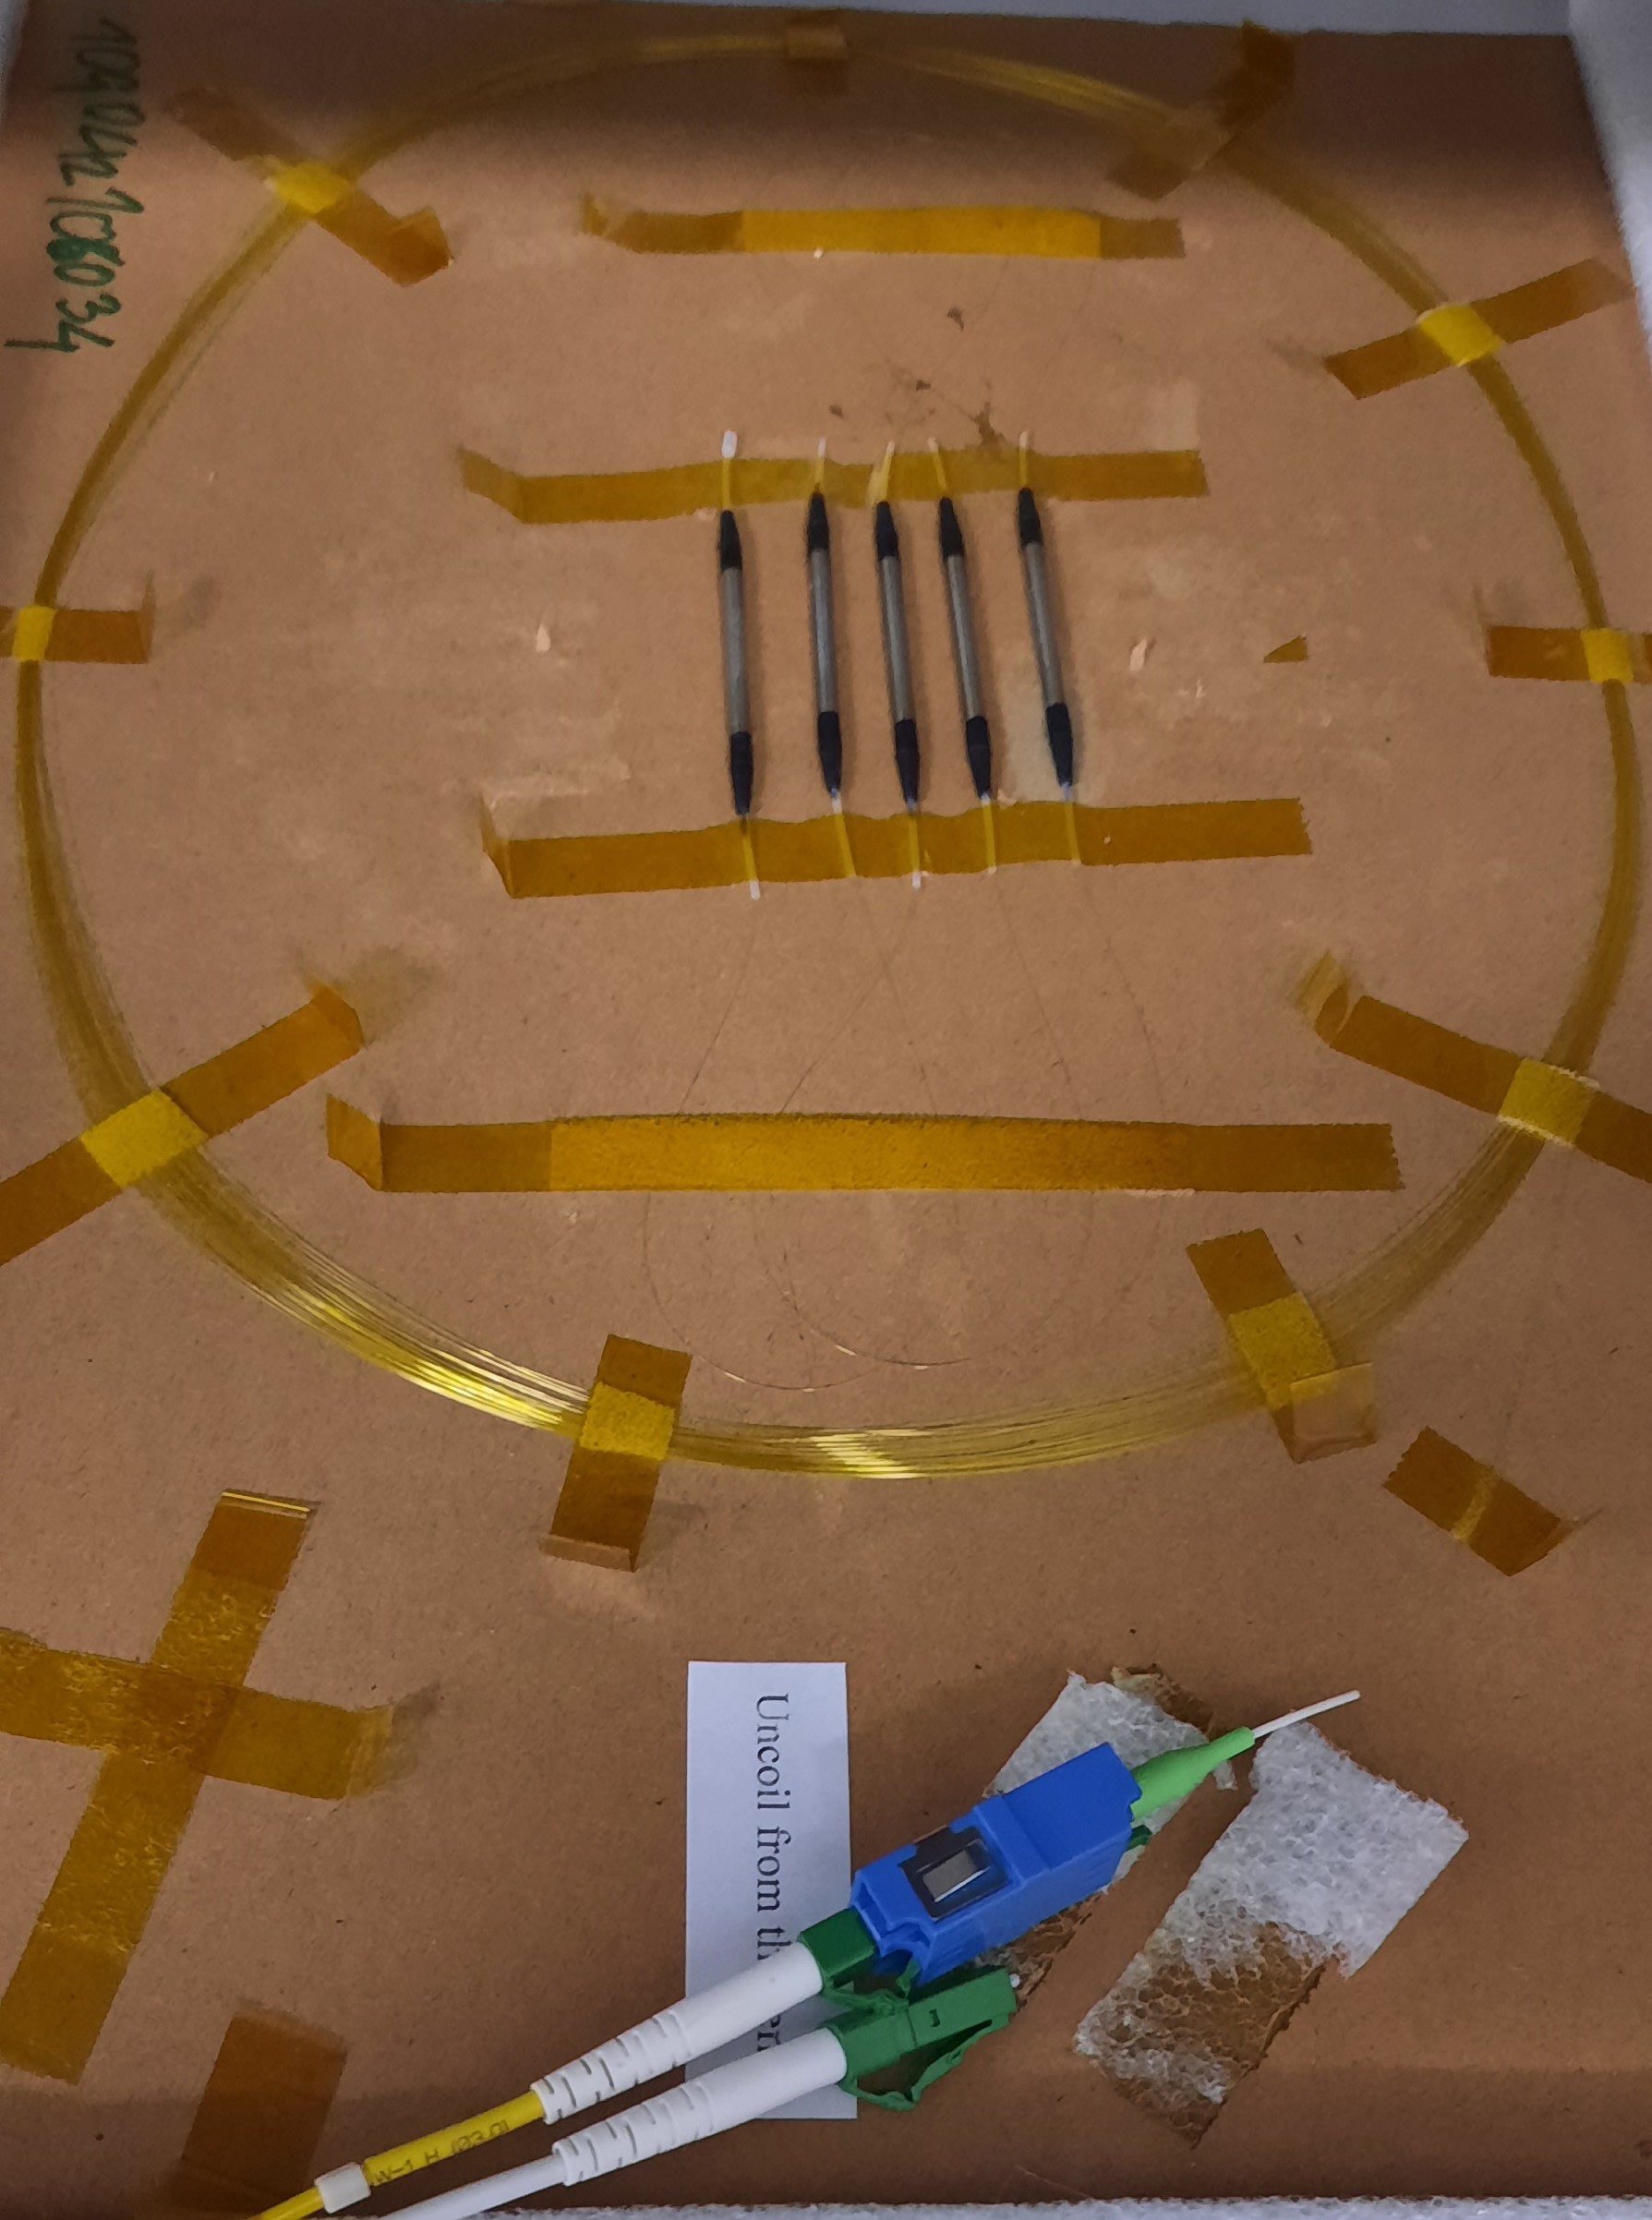
\includegraphics[angle=90,width=0.43\columnwidth]{Chapter5/images/t_array1.jpg}
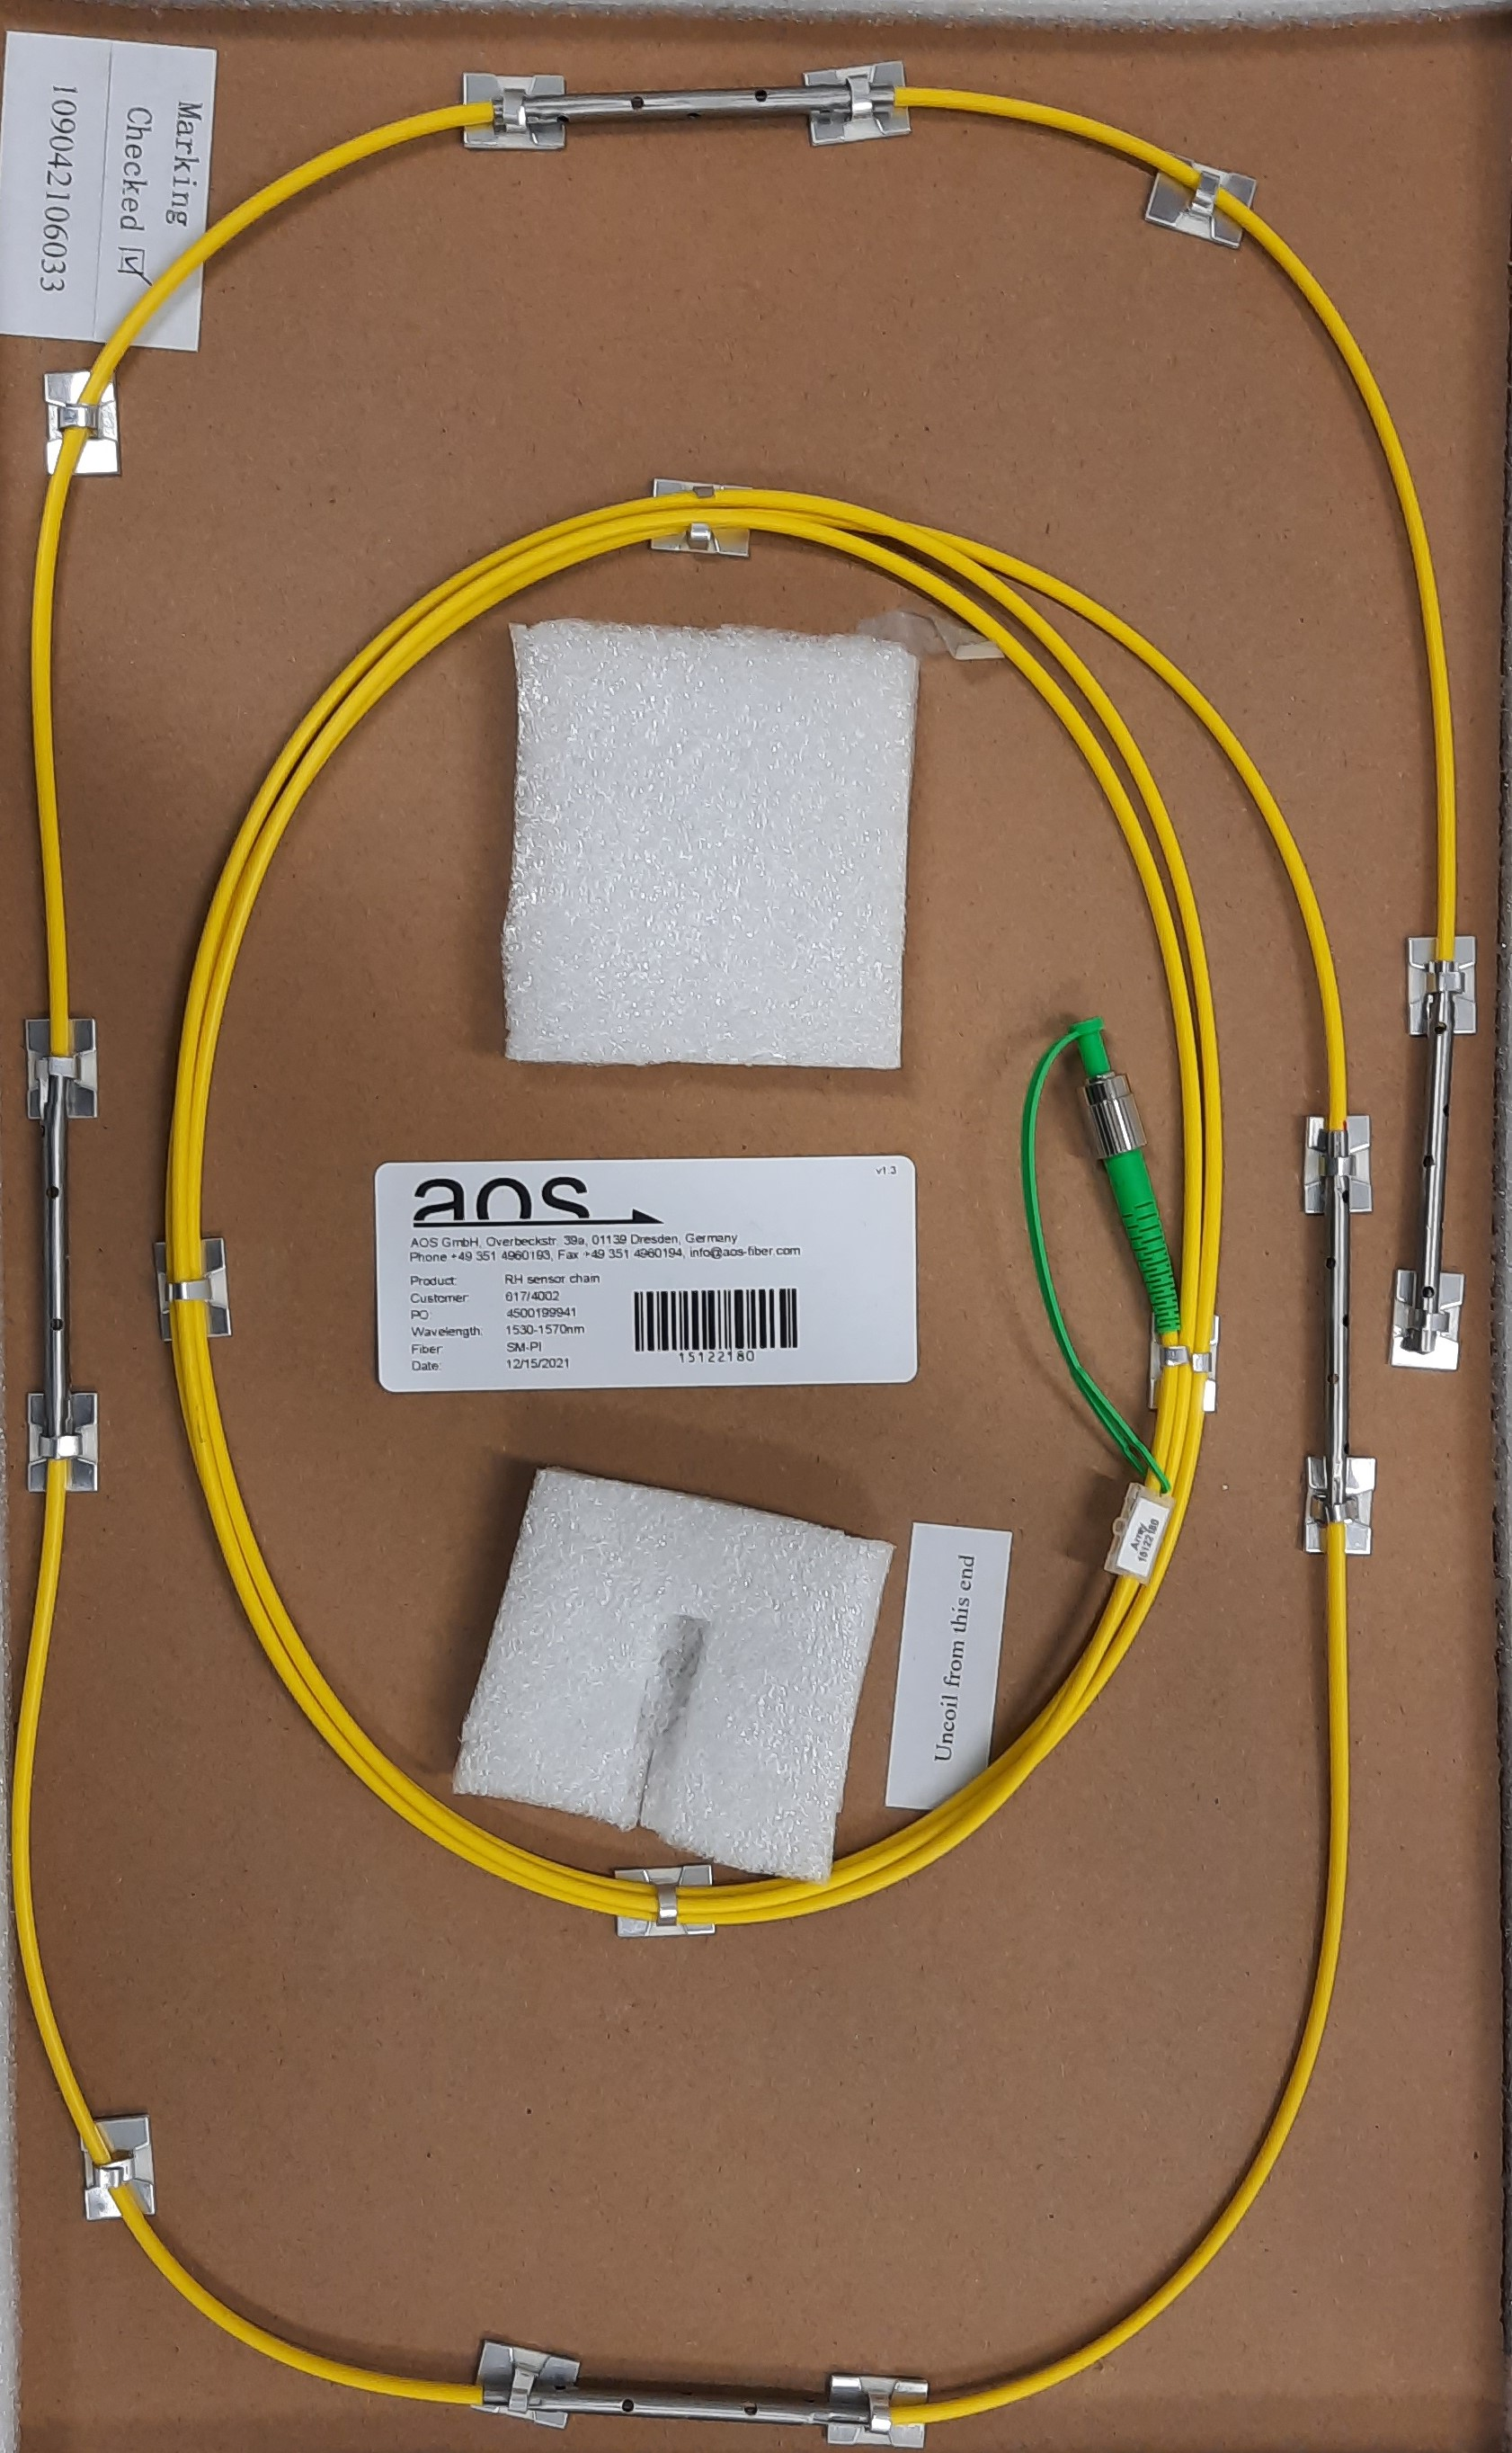
\includegraphics[angle=90,width=0.52\columnwidth]{Chapter5/images/rh_array1.jpg}
\caption{\gls{RH} and temperature sensing arrays. The fibers do not have the jacket applied on the polyimide coating. The left photo shows the temperature sensing array and the right one shows the \gls{RH} sensing array after packaging the FBG in strain-free conditions. The arrays were manufactured by Technica and packaged by AOS Electronics.}
\label{fig_single_photo}
\end{figure}

\section{Experimental setup}
The devices used to calibrate and characterize the sensors are listed in the figure~\ref{fig:fos_arch}. The sensors were calibrated using a S8000 chilled mirror hygrometer~\cite{michell_s8000}. Additionally, to compare the results two industrial \gls{RH} sensors were used: HYT221 and SHT85 (see section \ref{capacitive_sensors}. The temperature during the testing was controlled by a Binder MKF chamber~\cite{binder} which offers also relative humidity control down to \SI{0}{\celsius}. 
In general, two calibration methods were used to characterize the \gls{FBG}-based relative humidity sensors. The first method involved the use of different saturated salt solutions:
\begin{itemize}
    \item lithium chloride - \gls{RH} at \SI{25}{\celsius} 11 \%
    \item magnesium(II) chloride - \gls{RH} at \SI{25}{\celsius} 33 \%
    \item sodium chloride - \gls{RH} at \SI{25}{\celsius} 75 \%
\end{itemize}
Moreover, 100\% and 0\% conditions were achieved by using pure water and nitrogen flushing, respectively. Due to well-defined relative humidity values at a given temperature, this method offers a cost-effective way to calibrate a \gls{RH}. The second method relied on the humidity control (10\% to 80\% with a 10\% increment) of the climatic chamber.  The sensing instrument (light source) was the Micron Optics Hyperion SI255~\cite{si255}. The SI255 is a high power, low noise, ultra wide swept wavelength laser, it is guaranteed to provide absolute accuracy of 1~pm at every scan within the operating range of 1500 -- 1600~nm. 

The setup was controlled by the developed \gls{EPICS} based framework. The custom-written \glspl{IOC} were used to obtain data from the temperature and humidity sensors, as well as from the climatic chamber. The data related to the fiber optic sensors were collected through \footnote{ENLIGHT Sensing Analysis Software is a powerful utility that is included with Micron
Optics sensing interrogators.}{ENLIGHT} software, and a custom \gls{IOC} connected to it. Subsequently, all the data was stored using an archiver appliance to a Redis database. 

\begin{figure}[!h]
\centering
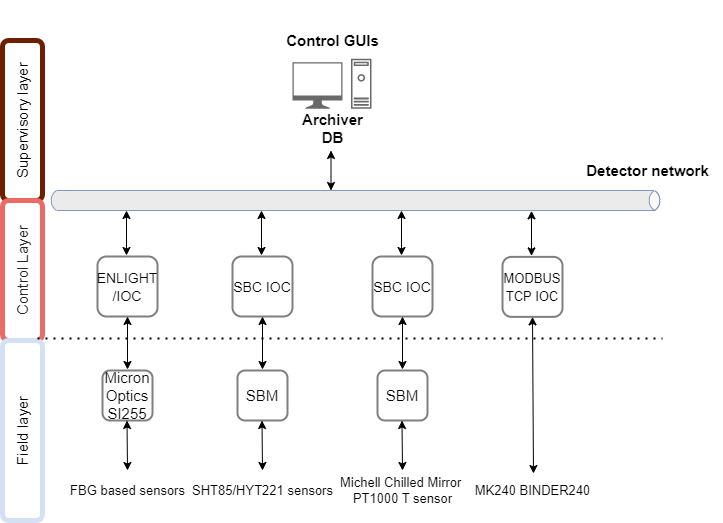
\includegraphics[width=0.75\columnwidth]{Chapter5/images/FOS_dcs_scheme.png}
\caption{Controls architecture for the temperature and humidity sensor measurement}
\label{fig:fos_arch}
\end{figure}
\subsection{Sensors characterization}
To characterize the sensors and estimate their uncertainty, it's necessary to know the wavelength reflected at the \gls{FBG}. The figure~\ref{fig_hygrometer1} shows an example of the readout of the SI255 device from the hygrometer. What's of interest is the center of the depicted pick and its intensity. To perform an accurate calibration of the sensors, the \gls{RH} and temperature sensitivity factors have to reside in precisely controlled environmental conditions. The climatic chamber offers the temperature control between \SI{-40}{\celsius} and \SI{180}{\celsius}. As both methods to control humidity offer only limited capabilities below \SI{0}{\celsius} for calibration of series production a new custom humidity control system will need to be considered~\cite{Berruti, Veldscholte:2021wjt}. 
\begin{figure}[!h]
\centering
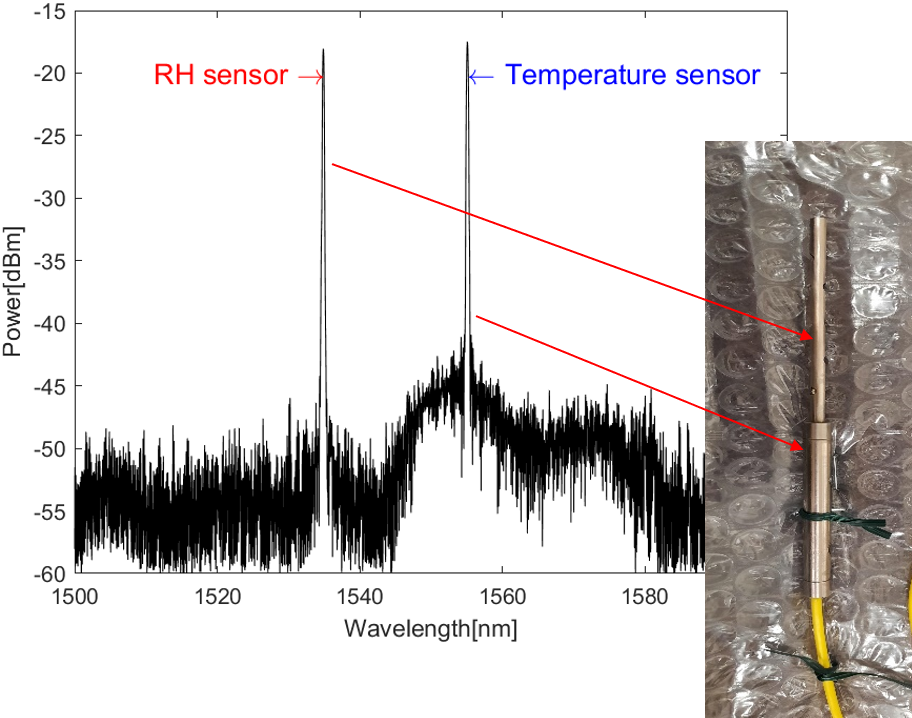
\includegraphics[width=0.6\columnwidth]{Chapter5/images/hygr.png}
\caption{The power of the FBG reflected wavelength. Each of the peaks is correlated with one of the gratings in the fiber.}
\label{fig_hygrometer1}
\end{figure}
One of the most important sensor characteristics is accuracy, which holds information about the deviation of the measured value from the ideal value. Overall, the accuracy is combined of several factors~\cite{sensors_physics}:
\begin{itemize}
    \item calibration error - a constant error over the whole range of measurements, its source is related to the accuracy of the reference device and the calibration method applied,
    \item hysteresis - a deviation of the sensor's output at a certain point of the input single when it is approached from opposite directions (see figure~\ref{fig:accuracy}), 
    \item non-linearity - in the characterization of the \glspl{FBG} it is assumed that the response of the sensors to the stimulus (increasing humidity or temperature) can be described by a straight line. Therefore, any deviation from the linearity is considered a contribution for the uncertainty,
    \item repeatability - the error caused by the inability of a sensor to represent the same value at the same conditions. 
\end{itemize}
\begin{figure}[!h]
\centering

\includegraphics[width=0.85\columnwidth]{Chapter5/images/Picture2.png}
\caption{Different contributions to the sensor's accuracy}
\label{fig:accuracy}
\end{figure}
Combining all the errors we can estimate the total uncertainty of a sensor, which is given as:
\begin{equation}
    \mu_{c} = \sqrt{\mu_{1}^{2} + \mu_{2}^{2} + ... + \mu_{i}^{2} + ... + \mu_{n}^{2}}
\end{equation}
In general, the total uncertainty of a \gls{FBG} sensor may consist of many other factors, including the uncertainty of the peak wavelength measurement etc. But the factors listed above were considered have the largest contribution. 

\section{Results}
\label{fbg_results}
In this section, the efforts to calibrate and characterize the humidity arrays and hygrometers are described in detail. The calibration relied on the Bragg wavelength shift measurements while increasing the \gls{RH} levels at a constant temperature value. This measurement was then repeated for different temperature values. It is a commonly used approach to estimate the humidity and temperature sensitivities~\cite{Berruti}. For the calibration using the saturated salt solutions, the sensors were exposed to the given salt for a prolonged time of about 6 hours. In the second case, the calibration step in the climatic chamber lasted about 2 hours. Keeping the sensors for this time at a constant conditions, ensured that the equilibrium is reached. 
\subsection{Characterization of RH FOS}
The test subjects were two hygrometers (\SI{15}{\micro\metre} PI coating) and  5 \gls{RH} sensors (\SI{20}{\micro\metre)} in an array with \SI{15}{\cm}. The spectral response of the sensor in the array can be in the figure~\ref{fig_array_wavelength}. The spectral responses are usually the first sign that the sensors perform correctly. 
\begin{figure}[!h]
\centering
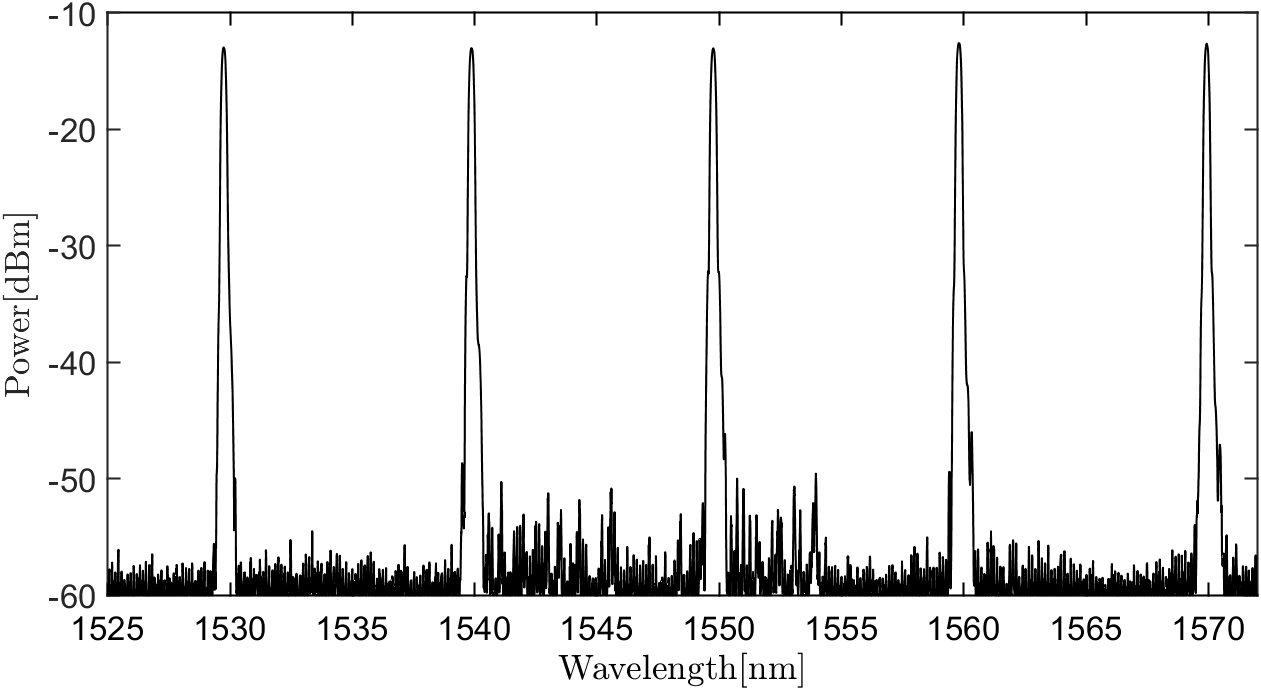
\includegraphics[width=0.85\columnwidth]{Chapter5/images/rh_array.png}
\caption{Spectral response of the relative humidity array.}
\label{fig_array_wavelength}
\end{figure}
The second test involved checking the humidity response in the range (10\% to 80\%), see figures~\ref{fig_response}. In both cases, increasing the relative humidity inside the test chamber results in the shift of the Bragg wavelength toward higher values. It's related to the increasing strain on the grating resulting from deposition of water molecules in the polyimide. These measurements were taken at a stable temperature of \SI{20}{\celsius}.
\begin{figure}[!h]
\centering
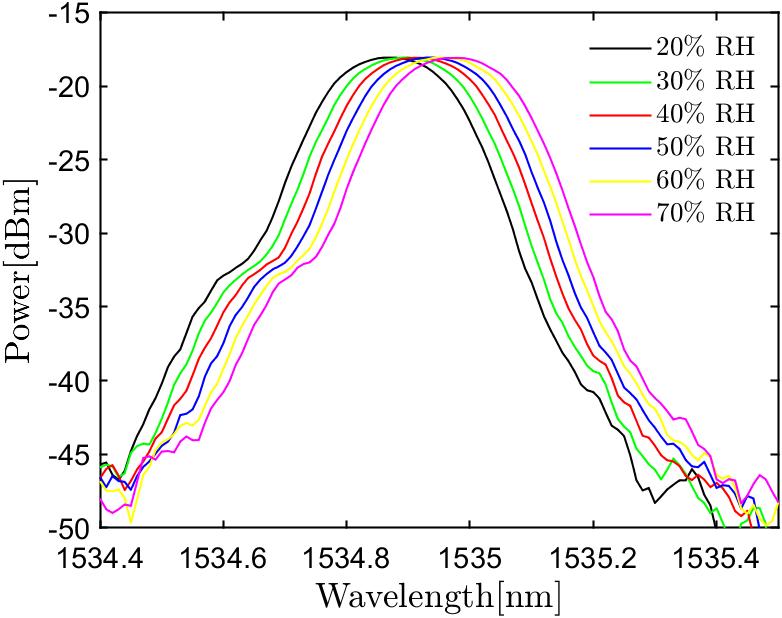
\includegraphics[width=0.45\columnwidth]{Chapter5/images/rh.png}
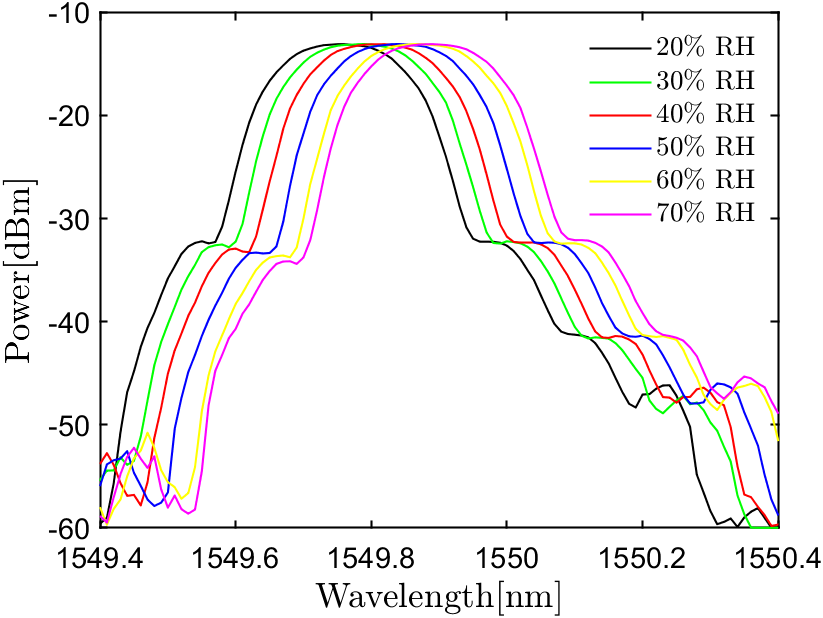
\includegraphics[width=0.47\columnwidth]{Chapter5/images/rh_array2.png}
\caption{Humidity induced Bragg wavelength shift of the hygrometer (left) and first sensor in the array (right). The spectral response is depicted as the power of the reflected wavelength. }
\label{fig_response}
\end{figure}
\newpage
Figures~\ref{fig_single_calibration} and~\ref{fig_array_calibration} depict the calibration curves of the hygrometer and one of the array sensors. The calibration curves were obtained by changing the humidity values from ~10\% up to 80\% at constant temperatures. The temperature range was from \SI{-20}{\celsius} to about \SI{30}{\celsius}. The figures depict a linear response to the humidity increase at every temperature. The measurements below \SI{0}{\celsius} have a relatively larger uncertainty, due to the limited humidity control and fewer points. Moreover, the change of temperature results also in the shift of the Bragg wavelength toward smaller values, what is also in acceptance with results from Kronenberg~\cite{Kronenberg:02} and Berruti~\cite{Berruti}. In the array calibration, two curves are missing, because the sensitivity factors had unrealistically high uncertainties. This is most likely caused by an additional strained applied to the sensors after handling. %The issue related to the array is discussed in the next sections.

\begin{figure}[!h]
\centering
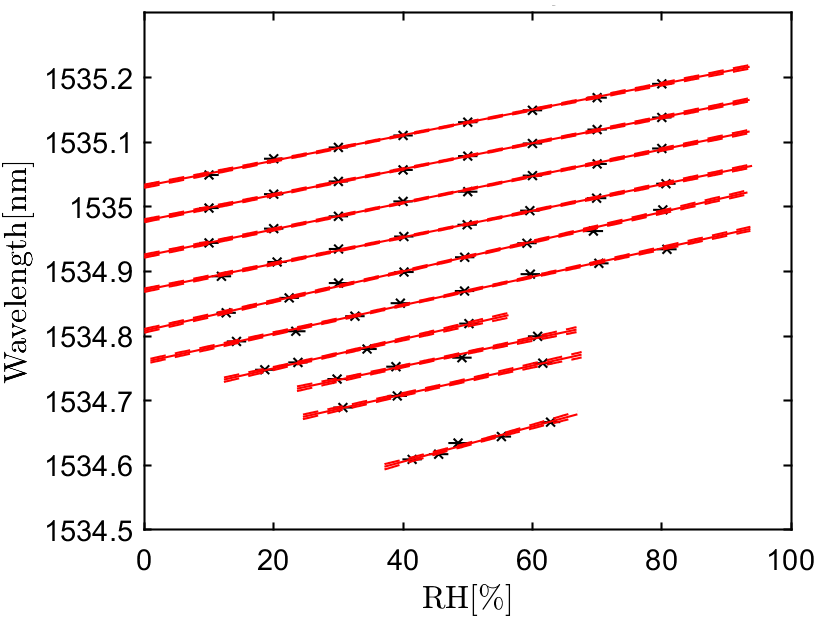
\includegraphics[width=0.8\columnwidth]{Chapter5/images/RHS.png}
\caption{Calibration curves for the hygrometer}
\label{fig_single_calibration}
\end{figure}

\begin{figure}[!h]
\centering
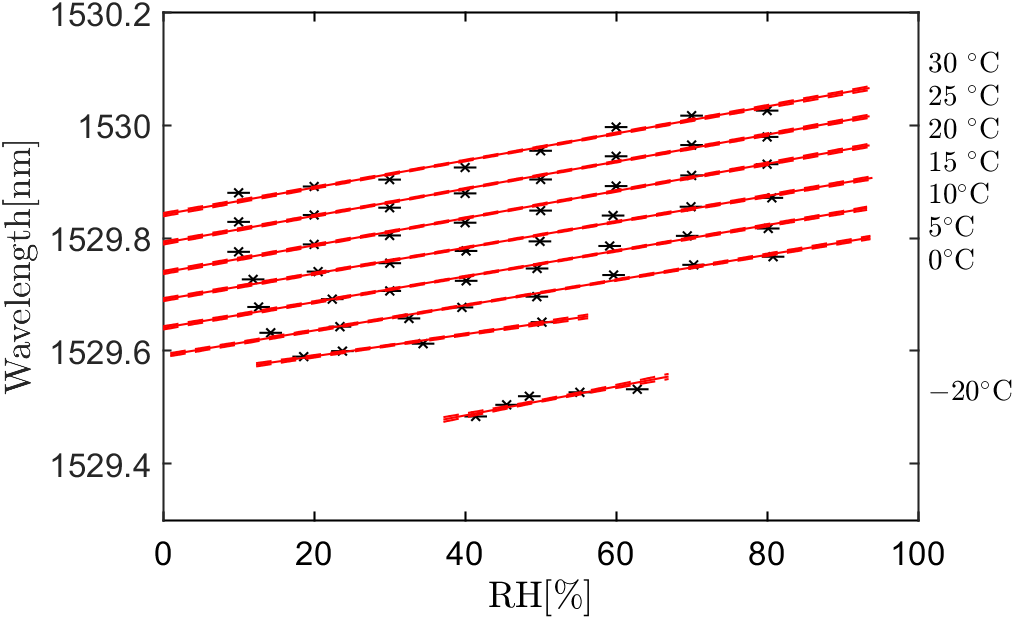
\includegraphics[width=0.8\columnwidth]{Chapter5/images/RH1.png}
\caption{Calibration curves for the first \gls{RH} sensor in the array}
\label{fig_array_calibration}
\end{figure}
\newpage
The uncertainties of the reference devices (the Michell chilled mirror and the PT1000 temperature sensors - \SI{0.001}{\celsius}) are taken into account, together with the calibration error of the linear fit. In this case, the errors were assumed to be following the Gaussian distribution and the confidence level of 68\%. The humidity sensitivity at different temperatures and their corresponding uncertainties are depicted in the~\ref{fig_RH_sens}. 

\begin{figure}[!h]
\centering
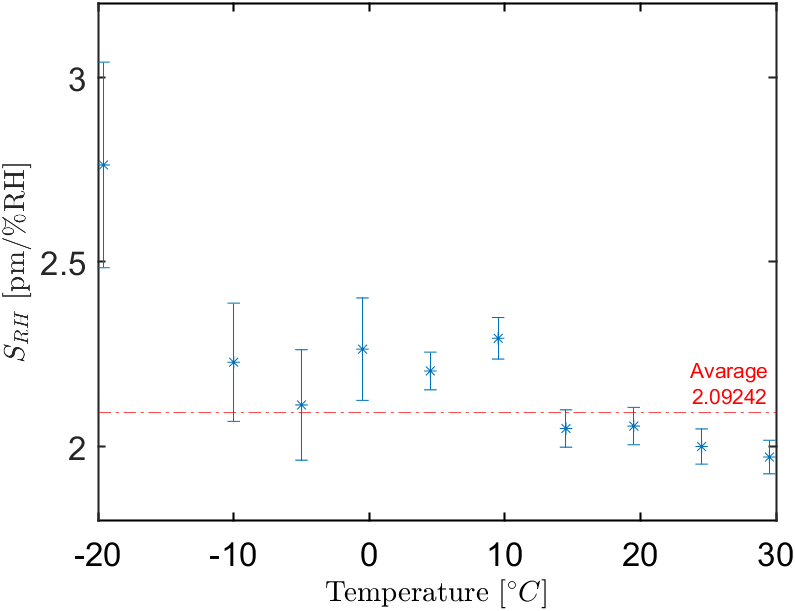
\includegraphics[width=0.55\columnwidth]{Chapter5/images/RHS_RH.png}
\caption{Humidity sensitivity at different temperatures with the corresponding uncertainty (hygrometer).}
\label{fig_RH_sens}
\end{figure}
\begin{figure}[!h]
\centering
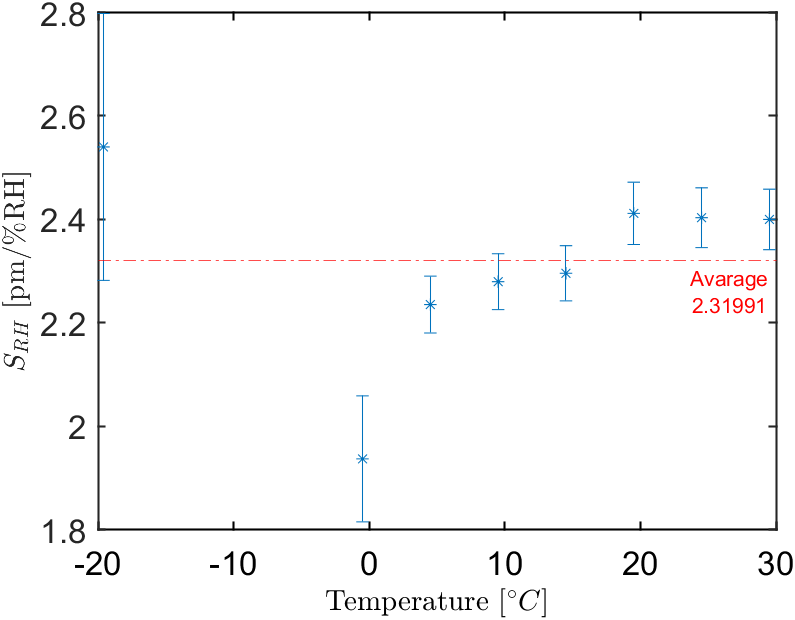
\includegraphics[width=0.55\columnwidth]{Chapter5/images/RH1_RH.png}
\caption{Humidity sensitivity at different temperatures with the corresponding uncertainty (first sensor in the array.}
\label{fig_RH_sens2}
\end{figure}
Similar plots were also obtained for all the other sensors inside the array (see figure~\ref{fig_calibration}. The second hygrometer didn't show a linear response to the changing conditions. That's why it's not included in the summary plots. Figure~\ref{fig_calibration} shows the humidity sensitivity of the calibrated \gls{RH} sensors. The average $S_{RH}$ for the array sensors is $2.77\pm0.03$~pm/\%RH  and $2.09\pm0.02$~pm/\%RH for the hygrometer. Given the uncertainty of the coating thickness, these results are in line with the findings from Yeo and Kronenberg~\cite{Kronenberg:02,YEO_PI}. The uncertainty obtained from the calibration is much smaller than the error introduced by the interrogator itself, which is $1$~pm. That means that the hygrometer measures with an accuracy of 0.5\%RH and for the array sensors on average $0.36$~\%RH. 
%RH
%R
\begin{figure}[!h]
\centering
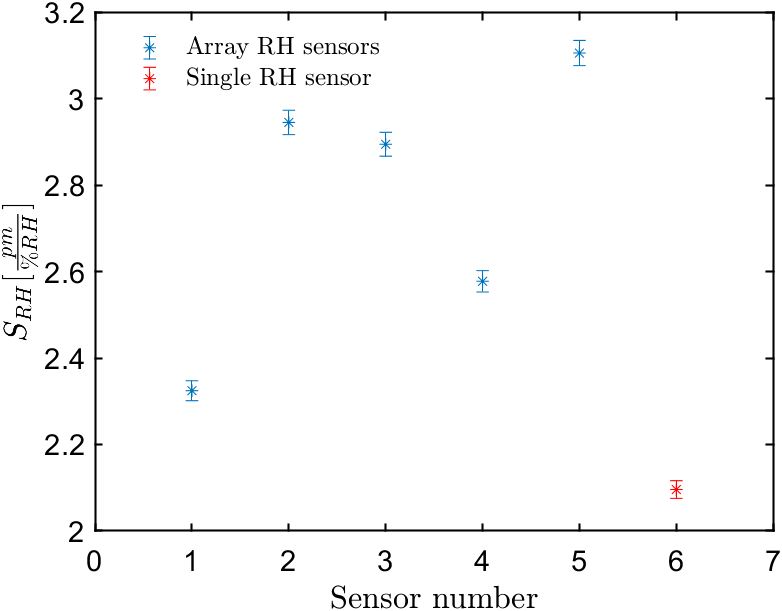
\includegraphics[width=0.6\columnwidth]{Chapter5/images/comp1.png}
\caption{Humidity sensitivity of the sensors with the corresponding uncertainty.}
\label{fig_calibration}
\end{figure}
The second coefficient called temperature sensitivity conveys information on how the wavelength shifts depending on the changing temperature. In this case for the stable \gls{RH} values, the temperature was changed between \SI{-20}{\celsius} or partially deduced from the humidity sensitivity curves. 
The average temperature sensitivity $S_\text{T}$ value for the array is $10.25\pm0.02\,\mathrm{\frac{pm}{^{\circ}C}}$ and for the hygrometer $10.87\pm 0.02\,\mathrm{\frac{pm}{^{\circ}C}}$ (see Figure~\ref{fig_calibration1}). The temperature sensitivity is about an order of magnitude larger than the humidity sensitivity. That implies that the temperature sensor located next to the \gls{RH} one should measure with good accuracy, in order to avoid a huge uncertainty of the humidity measurement. A \SI{0.1}{\celsius} temperature uncertainty leads to almost $0.5$~\%RH uncertainty in the case of the hygrometer and $0.36$~\%RH. 
\begin{figure}[!h]
\centering
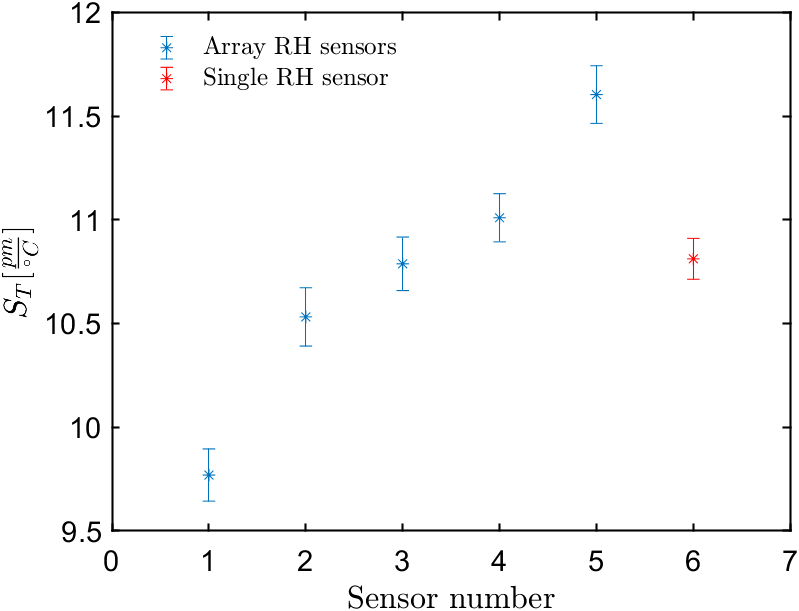
\includegraphics[width=0.6\columnwidth]{Chapter5/images/comp.png}
\caption{Temperature sensitivity of the sensors with the corresponding uncertainty.}
\label{fig_calibration1}
\end{figure}



\subsection{Time response}
The time response of the hygrometer and the array sensors was investigated. In principle, the \gls{FBG} based \gls{FOS} has a much longer time response to the capacitive sensors. The comparison of the time response of the different \gls{FOS} to the capacitive sensors (two SHT85 and HYT221 sensors). The time response of different sensors is often compared using for example the time to reach 63\% of targeted value $\tau_{63}$. Figures~\ref{fig_time_response} and~\ref{fig_time_response2} depict the comparison of the time response of the hygrometer and one of the array sensors with commercial capacitive sensors. 

\begin{figure}[!h]
\centering
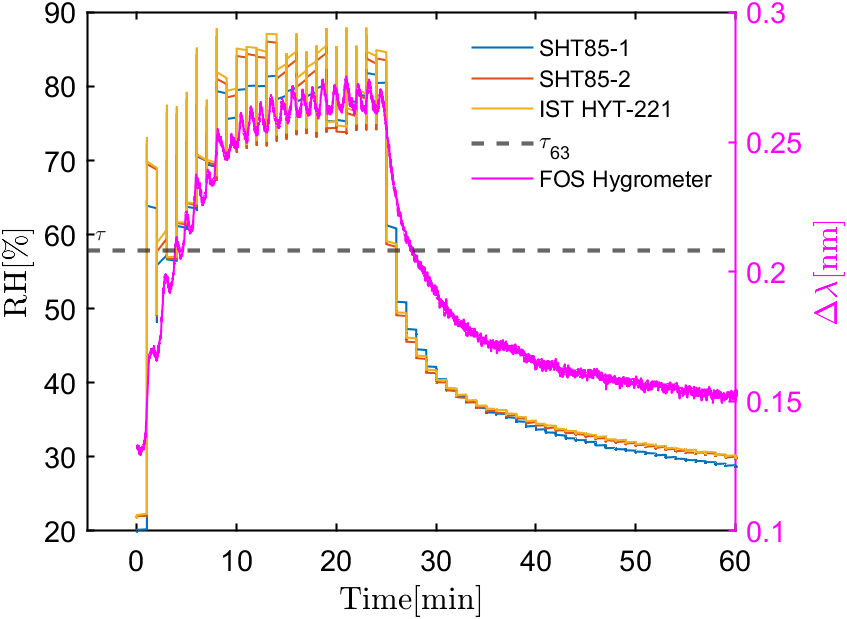
\includegraphics[width=0.47\columnwidth]{Chapter5/images/20responseRH.png}
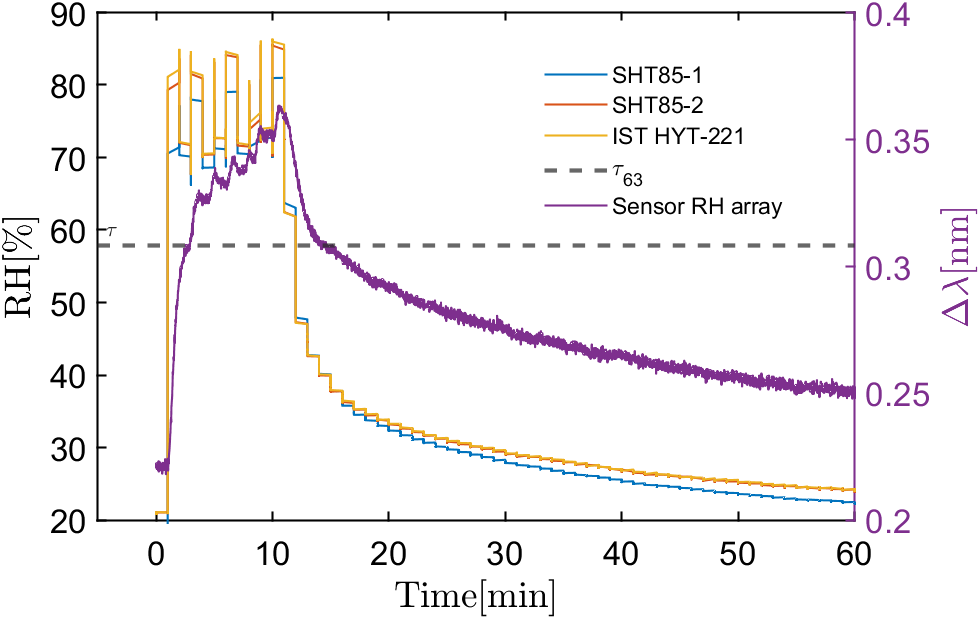
\includegraphics[width=0.47\columnwidth]{Chapter5/images/20responseRH2.png}
\caption{Time response of sensors}
\label{fig_time_response}
\end{figure}

\begin{figure}[!h]
\centering
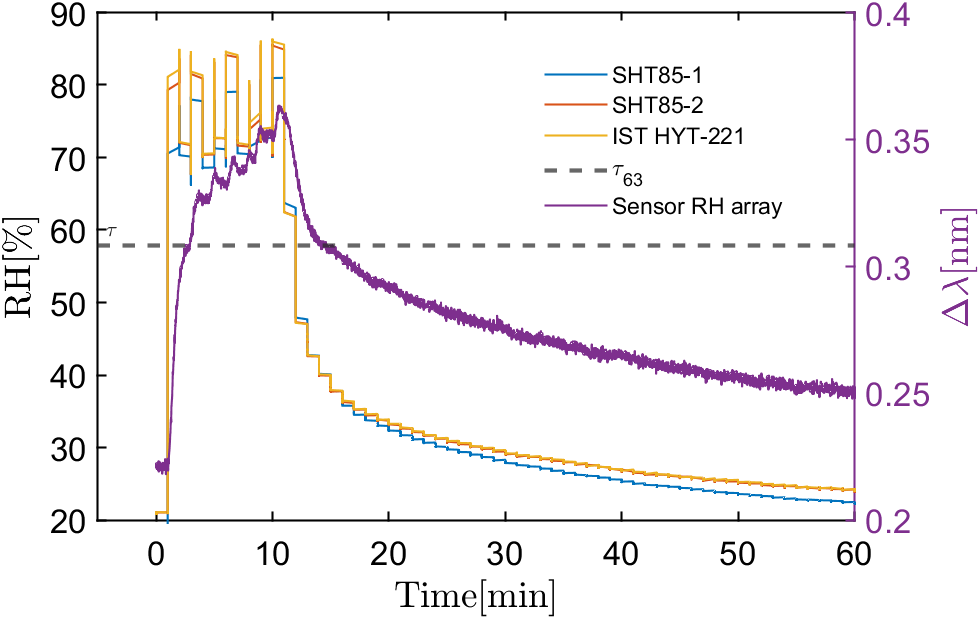
\includegraphics[width=0.47\columnwidth]{Chapter5/images/20responseRH2.png}
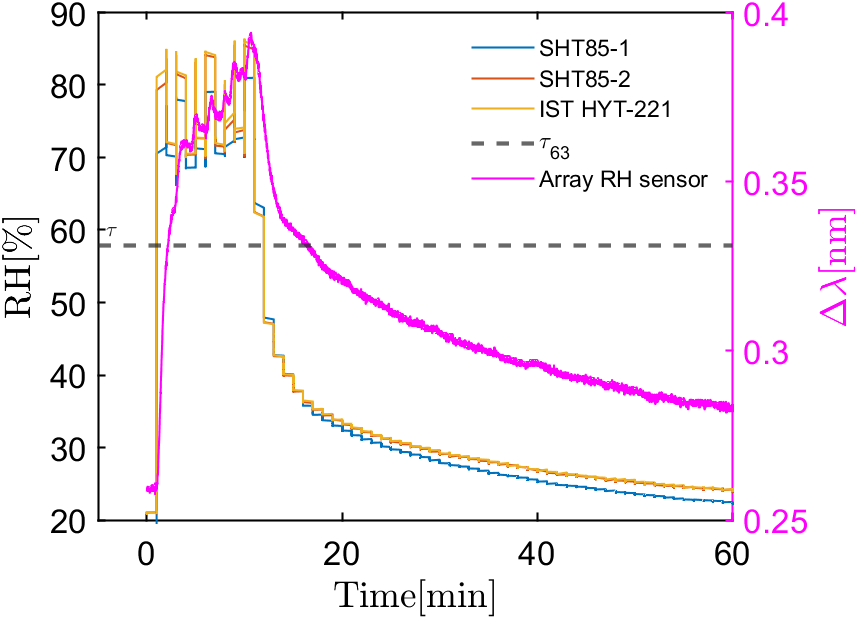
\includegraphics[width=0.47\columnwidth]{Chapter5/images/020responseRH2.png}
\caption{Time response of sensors}
\label{fig_time_response2}
\end{figure}


\subsection{Hysteresis}

\begin{figure}[!h]
\centering
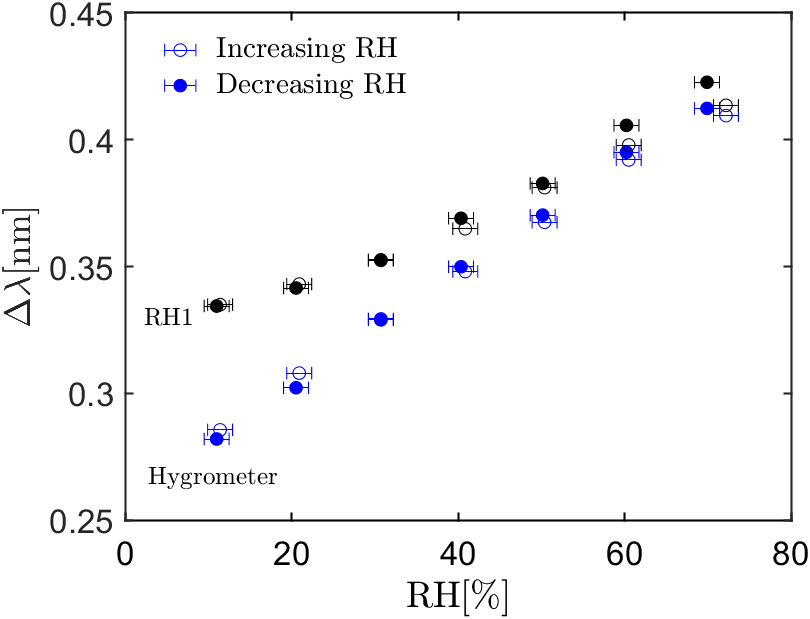
\includegraphics[width=0.6\columnwidth]{Chapter5/images/25_RHS.png}
\caption{Hysteresis}
\label{fig_hysteresis}
\end{figure}

\begin{figure}[!h]
\centering
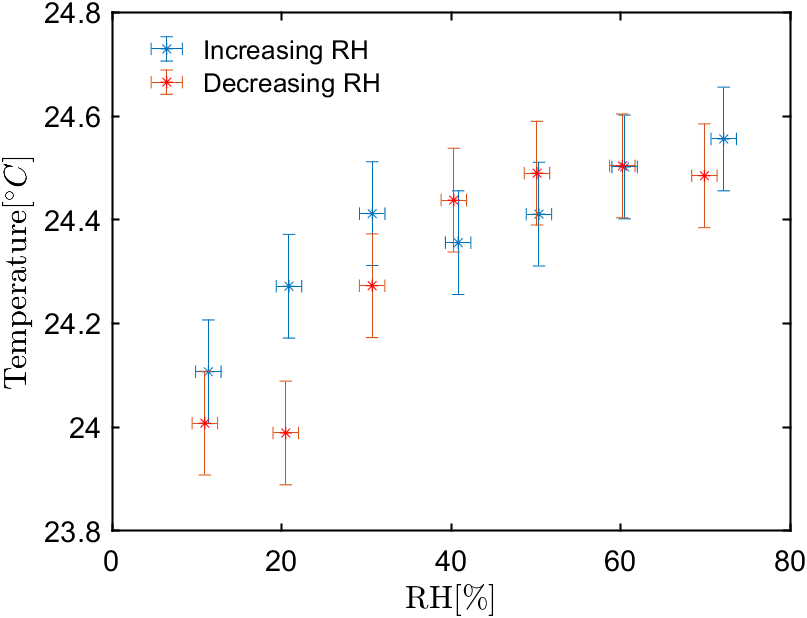
\includegraphics[width=0.6\columnwidth]{Chapter5/images/25_RHST.png}
\caption{Hysteresis}
\label{fig_hysteresis2}
\end{figure}



\subsection{Repeatability}


\begin{figure}[!h]
\centering
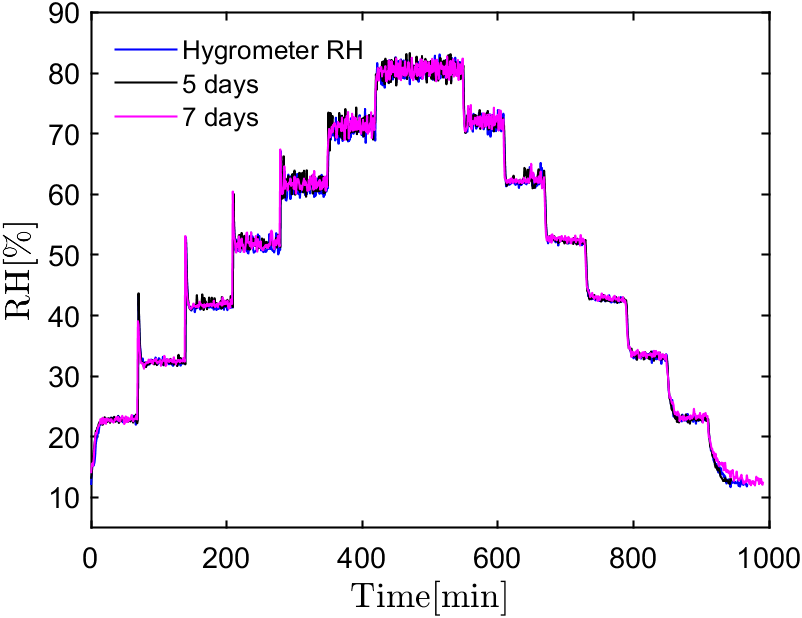
\includegraphics[width=0.6\columnwidth]{Chapter5/images/repeat.png}
\caption{Repeatability}
\label{fig_repeatability}
\end{figure}



\subsection{Conclusions}


\begin{figure}[!h]
\centering
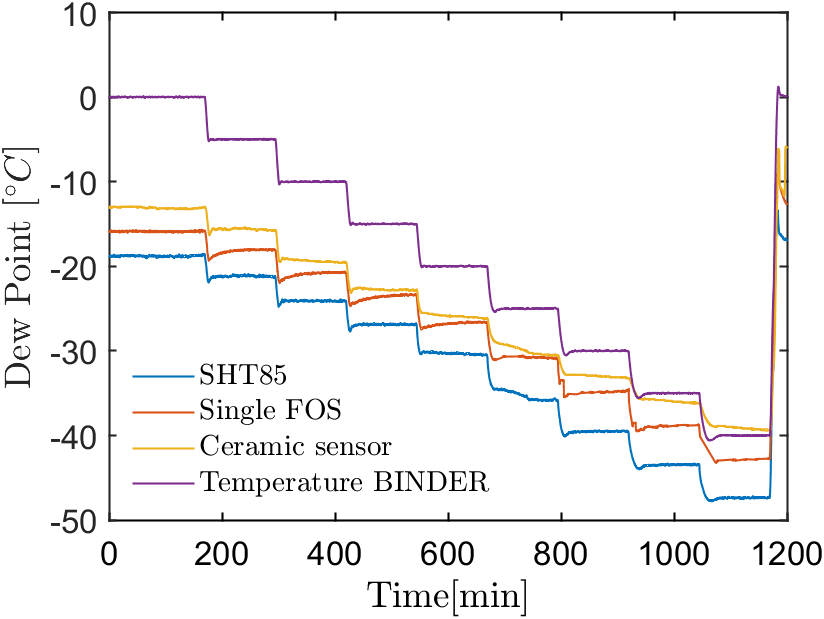
\includegraphics[width=0.6\columnwidth]{Chapter5/images/DPCPercent.png}
\caption{Comparison}
\label{fig_comparison}
\end{figure}

\begin{figure}[!h]
\centering
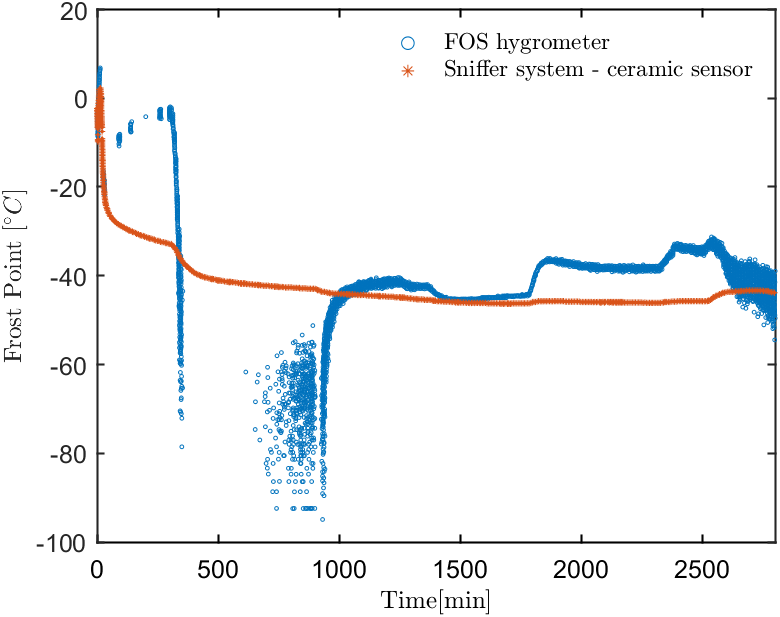
\includegraphics[width=0.6\columnwidth]{Chapter5/images/FOS_performance.png}
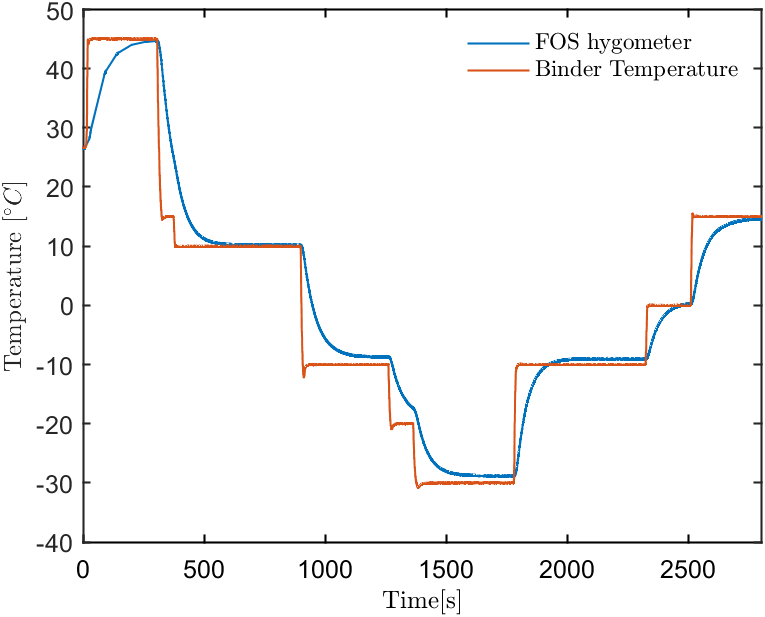
\includegraphics[width=0.6\columnwidth]{Chapter5/images/FOS_performance_T.png}
\caption{Comparison}
\label{fig_comparison1}
\end{figure}